%-------------------------------------------------------------------------------------------------%
\documentclass[12pt]{article}

%-------------------------------------------------------------------------------------------------%
\usepackage[spanish]{babel}
\usepackage[margin=1in]{geometry}
\usepackage[hidelinks]{hyperref}
\usepackage{amssymb,amsmath,amsthm,amsfonts}
\usepackage{enumerate}
\usepackage{graphicx}
\usepackage{datetime}
\usepackage{parskip}
\usepackage{apacite}
\usepackage{lipsum}
\usepackage{color}
\usepackage{float}
\usepackage{cancel}
\usepackage[framed,numbered,autolinebreaks,useliterate]{mcode}
%-------------------------------------------------------------------------------------------------%
\newenvironment{solution}{\begin{proof}[Solución]}{\end{proof}}
\renewcommand{\qedsymbol}{\rule{0.7em}{0.7em}}
\newtheorem{proposition}{Proposición}
\newtheorem{observation}{Observación}
\newtheorem{afirmation}{Afirmación}
\newtheorem{definition}{Definición}
\newtheorem{corollary}{Corolario}
\newtheorem{exercise}{Ejercicio}
\newtheorem{theorem}{Teorema}
\newtheorem{example}{Ejemplo}
\newtheorem{lemma}{Lema}
\graphicspath{{Img/}}
\decimalpoint
%-------------------------------------------------------------------------------------------------%
\title{Tarea 6 - Optimización No Lineal}
\author{Camara Medina Cynthia Lilian \\
Reyes Zamora Ollin \\
Alanis González Edzon Omar \\[0.2cm]
Mendoza Urrusquieta Jair Natael}
\date{\today}
%-------------------------------------------------------------------------------------------------%
\makeatletter
\let\thetitle\@title
\let\theauthor\@author
\let\thedate\@date
\makeatother
%-------------------------------------------------------------------------------------------------%
\begin{document}
%-------------------------------------------------------------------------------------------------%
\begin{titlepage}
\centering

\includegraphics[width=0.9\linewidth]{logo.png}\\[2.0 cm]
\textsc{\LARGE Escuela Superior de Física y Matemáticas}\\[1.2 cm]
\textsc{\Large Instituto Politécnico Nacional}\\[2.5 cm]
\rule{\linewidth}{0.2 mm} \\[0.4 cm]
{\huge \bfseries \thetitle}\\
\rule{\linewidth}{0.2 mm} \\[2.5 cm]
\textsc{\large \theauthor}
\vfill
{\large \thedate}
\end{titlepage}
%-------------------------------------------------------------------------------------------------%
\section{Método de Newton}
Aproximar el óptimo del siguiente problema mediante el método de Newton. Hacer las iteraciones "a mano". Comience las iteraciones en el punto $x^{(0)}=(-10,-10,10)$. No es necesario que reporte todos los cálculos ni todos los detalles, basta con poner resultados parciales de las iteraciones (no hacer más de cinco).

Minimizar 
\[f(x) = 3x_1^2+2x_2^2+x_3^2-2x_1x_2-2x_1x_3+2x_2x_3-6x_1-4x_2-2x_3\]

Definimos

\begin{itemize}

    \item $f=@(x) 3*x(1)^2+2*x(2)^2+x(3)^2-2*x(1)*x(2)-2*x(1)*x(3)+2*x(2)*x(3)-6*x(1)-4*x(2)-2*x(3)$
    \item $x0=[10,-10,10]$
    \item $e=0.001$
    \item MNewtondk(f,x0,e)
\end{itemize} 

El resultado fue:

\textbf{Iteracion 1}

vector \[gk = \begin{bmatrix}
    -54.00 & 44.00 & 22.00 
\end{bmatrix}^T\]

vector $H=$

\[
\begin{bmatrix}
    6.0000 &  -2.0000  & -2.0000\\
    -2.0000   & 4.0000  &  2.0000\\
    -2.0000   & 2.0000  &  2.0000\\
\end{bmatrix}
\] 

Resolvemos el sistema de ecuaciones dado por $H=dk$

\[
    dk=  \begin{bmatrix}
        -7.9999  & 11.0000 &   -7.9999
    \end{bmatrix}  
\]


Entonces calculamos $x^1 = x^0+dk$

\[
    x^1=    \begin{bmatrix}
        2.0001   & 1.0000   & 2.0001
    \end{bmatrix}
\]

Calculamos el nuevo gradiente $g(1)$

\[
    g(1)= \begin{bmatrix}
        0.2702 &   0.0219 &    0.0053
    \end{bmatrix}
\]

\[
    k^1=[255,1]^T
\]
\[
    ans = \begin{bmatrix}
        2.0001  & 1.0000  & 2.0001
    \end{bmatrix}
\]

Probando así que este método encuentra en una sola iteración el mínimo global de cualquier función cuadrática.

\section{Comprobación de Métodos}
\subsection{Newton vs Cauchy}

Programar en Octave (o Matlab) el método de Newton, que vimos en clase, para aproximar el mínimo del siguiente problema:
	\[f(x_1,x_2)=\left(x_2-\dfrac{5.1}{4\pi^2}x_1^2+\dfrac{5x_1}{\pi}-6\right)^2+10\left(1-\dfrac{1}{8\pi}\right)cos(x_1)+10\]
	
\subsubsection*{Iteración 1}
		
		Calculamos el vector Gradiente para posteriormente calcular el vector dirección gk.
		
		\begin{center}
			$V_{gk}=-g(x_0)=[-748.95\hspace{0.5cm} 31.98]^T$			
		\end{center}
	
		Calculamos la Hessiana evaluada en el punto $x_0$.
		
		\begin{center}
			$H(x_0)=\left[\begin{array}{cc}
				1.9137 & -0.0472\\
				-0.0472 & 0.0020
				\end{array}\right]$		
		\end{center}
	
		Ahora resolvemos el sistema de ecuaciones dado por $H(x_0)[x\ y]^T=V_{gk}$ para obtener $d_k$.
		
		\begin{center}
			$\begin{array}{ccc}
			1.9137x & -0.0472y & =-748.95\\
			-0.0472x & 0.0020y & =31.98
		\end{array}$
	
		$d_k=[0.0064\hspace{0.5cm}16.1436]$
		\end{center}	
		
		Calculamos $x_1=x_0+d_k$ y posteriormente calculamos el nuevo vector gradiente $g(x_1)$
		
		\begin{center}
			$x_1=[1.0064\hspace{0.5cm}17.1436]$
			
			$g(x_1)=[-5.1064\hspace{0.5cm}-0.0010]$
		\end{center}
	
	
	
        \subsubsection*{Iteración 2}
	
	Calculamos el vector Gradiente para posteriormente calcular el vector dirección gk.
	
	\begin{center}
		$V_{gk}=-g(x_1)=[5.11 \hspace{0.5cm} 0]^T$			
	\end{center}
	
	Calculamos la Hessiana evaluada en el punto $x_1$.
	
	\begin{center}
		$H(x_1)=\left[\begin{array}{cc}
			1.1241   & -0.0475\\
			-0.0475  & 0.0020
		\end{array}\right]$		
	\end{center}
	
	Ahora resolvemos el sistema de ecuaciones dado por $H(x_1)[x\ y]^T=V_{gk}$ para obtener $d_k$.
	
	\begin{center}
		$\begin{array}{ccc}
			1.1241x & -0.0472y & =5.11\\
			-0.0472x & 0.0020y & =0
		\end{array}$
		
		$d_k=[-1.7205\hspace{0.5cm} -40.8419]$
	\end{center}	
	
	Calculamos $x_2=x_1+d_k$ y posteriormente calculamos el nuevo vector gradiente $g(x_2)$
	
	\begin{center}
		$x_2=[-0.7141\hspace{0.5cm}-23.6984]$
		
		$g(x_2)=[-1.4535\hspace{0.5cm}-0.0745]$
	\end{center}

    \subsubsection*{Iteración 3}
	
	Calculamos el vector Gradiente para posteriormente calcular el vector dirección gk.
	
	\begin{center}
		$V_{gk}=-g(x_2)=[1453.51 \hspace{0.5cm} 74.50]^T$			
	\end{center}
	
	Calculamos la Hessiana evaluada en el punto $x_2$.
	
	\begin{center}
		$H(x_2)=\left[\begin{array}{cc}
			2.6356   & 0.0391\\
			0.0391   & 0.0020
		\end{array}\right]$		
	\end{center}
	
	Ahora resolvemos el sistema de ecuaciones dado por $H(x_2)[x\ y]^T=V_{gk}$ para obtener $d_k$.
	
	\begin{center}
		$\begin{array}{ccc}
			2.6356x & 0.0391y & =1453.51\\
			0.0391x & 0.0020y & =74.50
		\end{array}$
		
		$d_k=[-0.0021 \hspace{0.5cm} 37.2912]$
	\end{center}	
	
	Calculamos $x_3=x_2+d_k$ y posteriormente calculamos el nuevo vector gradiente $g(x_3)$
	
	\begin{center}
		$x_3=[-0.7161\hspace{0.5cm}13.59291]$
		
		$g(x_3)=[3.9668\hspace{0.5cm}-0.0010]$
	\end{center}

    \subsubsection*{Iteración 4}
	
	Calculamos el vector Gradiente para posteriormente calcular el vector dirección gk.
	
	\begin{center}
		$V_{gk}=-g(x_3)=[-3.97 \hspace{0.5cm} 0]^T$			
	\end{center}
	
	Calculamos la Hessiana evaluada en el punto $x_3$.
	
	\begin{center}
		$H(x_3)=\left[\begin{array}{cc}
			764.6380  &  39.2273\\
			39.2273   & 2
		\end{array}\right]$		
	\end{center}
	
	Ahora resolvemos el sistema de ecuaciones dado por $H(x_3)[x\ y]^T=V_{gk}$ para obtener $d_k$.
	
	\begin{center}
		$\begin{array}{ccc}
			764.6380x &39.2273y & =-3.97\\
			39.2273x & 2y & =0
		\end{array}$
		
		$d_k=[0.8387  \hspace{0.5cm} -16.4499]$
	\end{center}	
	
	Calculamos $x_4=x_3+d_k$ y posteriormente calculamos el nuevo vector gradiente $g(x_4)$
	
	\begin{center}
		$x_4=[0.1226\hspace{0.5cm}-2.8570]$
		
		$g(x_4)=[25.6962\hspace{0.5cm}-17.7020]$
	\end{center}


    \subsubsection*{Iteración 5}
	
	Calculamos el vector Gradiente para posteriormente calcular el vector dirección gk.
	
	\begin{center}
		$V_{gk}=-g(x_4)=[-25.70 \hspace{0.5cm}17.70]^T$			
	\end{center}
	
	Calculamos la Hessiana evaluada en el punto $x_4$.
	
	\begin{center}
		$H(x_4)=\left[\begin{array}{cc}
			443.9710   &  -2.9896\\
			-2.9896   & 2
		\end{array}\right]$		
	\end{center}
	
	Ahora resolvemos el sistema de ecuaciones dado por $H(x_4)[x\ y]^T=V_{gk}$ para obtener $d_k$.
	
	\begin{center}
		$\begin{array}{ccc}
			443.9710x &-2.9896y & =-25.70\\
			-2.9896x & 2y & =17.70
		\end{array}$
		
		$d_k=[0.0017\hspace{0.5cm}8.8536]$
	\end{center}	
	
	Calculamos $x_5=x_4+d_k$ y posteriormente calculamos el nuevo vector gradiente $g(x_5)$
	
	\begin{center}
		$x_5=[0.1243\hspace{0.5cm} 5.9966]$
		
		$g(x_5)=[-0.7530 \hspace{0.5cm}-0.0001]$
	\end{center}
	
	
    \subsubsection*{Iteración 6}
	
	Calculamos el vector Gradiente para posteriormente calcular el vector dirección gk.
	
	\begin{center}
		$V_{gk}=-g(x_5)=[0.75 \hspace{0.5cm}0]^T$			
	\end{center}
	
	Calculamos la Hessiana evaluada en el punto $x_5$.
	
	\begin{center}
		$H(x_5)=\left[\begin{array}{cc}
			-1.2741  & -3.0772\\
			-3.0772   & 2
		\end{array}\right]$		
	\end{center}
	
	Ahora resolvemos el sistema de ecuaciones dado por $H(x_5)[x\ y]^T=V_{gk}$ para obtener $d_k$.
	
	\begin{center}
		$\begin{array}{ccc}
			-1.2741x &-3.0772y & =0.75\\
			-3.0772x & 2y & =0
		\end{array}$
		
		$d_k=[-0.1253\hspace{0.5cm}-0.1928]$
	\end{center}	
	
	Calculamos $x_6=x_5+d_k$ y posteriormente calculamos el nuevo vector gradiente $g(x_6)$
	
	\begin{center}
		$x_6=[-0.0010 \hspace{0.5cm}5.8038]$
		
		$g(x_6)=[-0.6336\hspace{0.5cm}-0.3956]$
	\end{center}
	
	
    \subsubsection*{Iteración 7}
	
	Calculamos el vector Gradiente para posteriormente calcular el vector dirección gk.
	
	\begin{center}
		$V_{gk}=-g(x_6)=[0.63 \hspace{0.5cm}0.4]^T$			
	\end{center}
	
	Calculamos la Hessiana evaluada en el punto $x_6$.
	
	\begin{center}
		$H(x_6)=\left[\begin{array}{cc}
			9.0884  & 3.2313\\
			3.2313 & 2
		\end{array}\right]$		
	\end{center}
	
	Ahora resolvemos el sistema de ecuaciones dado por $H(x_6)[x\ y]^T=V_{gk}$ para obtener $d_k$.
	
	\begin{center}
		$\begin{array}{ccc}
			9.0884x &3.2313y & =0.63\\
			3.2313x & 2y & =0.4
		\end{array}$
		
		$d_k=[-0.0015\hspace{0.5cm}0.2002]$
	\end{center}	
	
	Calculamos $x_7=x_6+d_k$ y posteriormente calculamos el nuevo vector gradiente $g(x_7)$
	
	\begin{center}
		$x_7=[-0.0010 \hspace{0.5cm}5.8038]$
		
		$g(x_7)=[-0.0025\hspace{0.5cm}6.0040]$
	\end{center}

    \subsubsection*{Iteración 8}
	
	Calculamos el vector Gradiente para posteriormente calcular el vector dirección gk.
	
	\begin{center}
		$V_{gk}=-g(x_7)=[-0.01 \hspace{0.5cm}0]^T$			
	\end{center}
	
	Calculamos la Hessiana evaluada en el punto $x_6$.
	
	\begin{center}
		$H(x_6)=\left[\begin{array}{cc}
			-0.6289& 3.3043\\
		    3.3043& 2
		\end{array}\right]$		
	\end{center}
	
	Ahora resolvemos el sistema de ecuaciones dado por $H(x_6)[x\ y]^T=V_{gk}$ para obtener $d_k$.
	
	\begin{center}
		$\begin{array}{ccc}
			-0.6289x &3.3043y & =0.01\\
			3.3043x & 2y & =0
		\end{array}$
		
		$d_k=[0.0025\hspace{0.5cm}-0.0040]$
	\end{center}	
	
	Calculamos $x_8=x_7+d_k$ y posteriormente calculamos el nuevo vector gradiente $g(x_8)$
	
	\begin{center}
		$x_8=[-0.0000  \hspace{0.5cm} 5.9999]$
		
		$g(x_8)=[-0.1937 \hspace{0.5cm}-0.1452]$
		
		$\therefore x^*=[0,6]$
	\end{center}


Como nos dimos cuenta el programa de newton lo realizó en 8 iteraciones las cuales son muy pocas, sin embargo con el método de Cauchy es todo lo contrario puesto que alcanzamos unas iteraciones exhorbitantes, agregaremos una imagen como muestra de lo dicho anteriormente pero aun así si se llega al mismo resultado.
\begin{figure}[H]
    \centering
    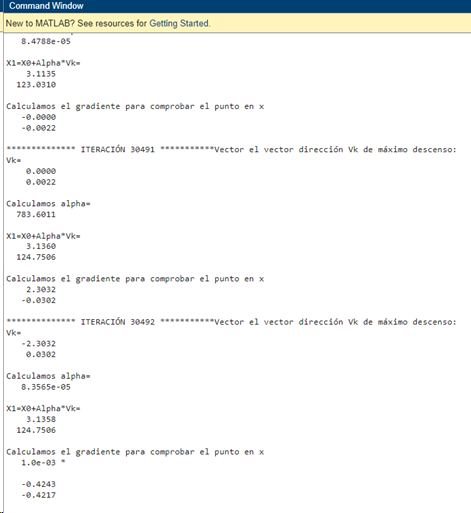
\includegraphics[height = 6cm]{resultados_MP.png}
    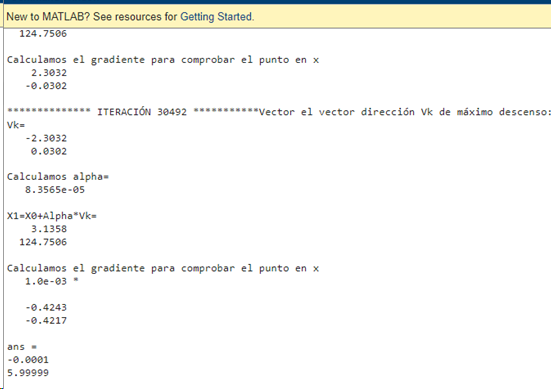
\includegraphics[height = 6cm]{resultados_MP1.png}
\end{figure}

\section{Multistart}

\begin{enumerate}
    \item Genere 2500 puntos uniformemente distribuidos en $[-5, 10] \times [0, 15]$. Tome cada uno de estos puntos como punto inicial y pruebe sus programas del inciso anterior (Newton y pendiente máxima). Reporte cuántos y cuáles óptimos distintos se hallaron en total.
    
    Los puntos generados distintos por el programa son:
    \begin{itemize}
        \item Newton
        \[\begin{bmatrix}
            -182.22          &         4585.09 \\
            -182.22          &          4585.1\\
            -166.51          &         3852.47\\
            -147.66          &         3057.47\\
            -131.95          &          2465.1\\
            -125.67          &            2246\\
            -122.53          &         2140.27\\
            -103.68          &         1559.47\\
             -97.39          &         1386.27\\
             -84.83          &         1070.47\\
             -72.26          &          795.47\\
              -59.7          &          561.27\\
             -56.55          &           509.1\\
             -53.41          &          459.47\\
             -50.27          &           412.4\\
             -40.85          &          286.47\\
              -37.7          &           249.6\\
             -34.56          &          215.27\\
             -31.42          &          183.49\\
             -28.28          &          154.27\\
             -25.14          &          127.59
            \end{bmatrix}
            \begin{bmatrix}
                -25.14          &           127.6 \\
                -22          &          103.47\\
             -18.85          &           81.89\\
             -18.85          &            81.9\\
             -15.71          &           62.87\\
             -12.57          &           46.39\\
             -12.57          &            46.4\\
              -9.43          &           32.47\\
              -6.29          &           21.09\\
              -6.29          &            21.1\\
              -3.15          &           12.27\\
              -0.01          &            5.99\\
              -0.01          &               6\\
                  0          &            5.99\\
                  0          &               6\\
               3.14          &            2.27\\
               6.28          &            1.09\\
               6.28          &             1.1\\
               9.42          &            2.47\\
              12.56          &            6.39\\
              12.56          &             6.4
            \end{bmatrix}
            \begin{bmatrix}
               15.7          &           12.87\\
              18.84          &           21.89\\
              18.84          &            21.9\\
              21.99          &           33.47\\
              25.13          &           47.59\\
              28.27          &           64.27\\
              34.55          &          105.27\\
              37.69          &          129.59\\
              37.69          &           129.6\\
              40.84          &          156.47\\
              43.98          &          185.89\\
              43.98          &           185.9\\
              47.12          &          217.87\\
               53.4          &          289.47\\
              56.54          &           329.1\\
              62.83          &          415.99\\
              62.83          &             416\\
              65.97          &          463.27\\
              87.96          &           865.6\\
             109.95          &         1392.87\\
             113.09          &          1478.4\\
             226.19          &         6255.59\\
        \end{bmatrix}\]
        \item Pendiente Maxima 
        \[\begin{bmatrix}
            -15.71           &          62.87 \\
            -3.15            &         12.27\\
            21.99            &         33.47\\
        \end{bmatrix}\]
    \end{itemize}
    \item Compare el número (promedio sobre los 2500 puntos) de evaluaciones
    de la función objetivo utilizadas para obtener los óptimos con cada
    algoritmo, cuente cuántas veces se calculó el gradiente de la función
    objetivo y cuántas veces la matríz Hessiana en cada caso.

    Llamadas promedio a la función
    \begin{itemize}
        \item Newton
        \begin{itemize}
            \item Llamadas a la función: 87.9
            \item Llamadas a la gradiente: 4.3
            \item Llamadas a la hessiana: 4.3
        \end{itemize}
        \item Pendiente Maxima
        \begin{itemize}
            \item Llamadas a la función: 302.7
            \item Llamadas a la gradiente: 75.4
            \item Llamadas a la hessiana: 0
        \end{itemize}
    \end{itemize}
    \item Escriba sus conclusiones.
    
    El método de Newton genera más puntos que el método de Pendiente Máxima, sin embargo, estos no son los óptimos de la función pues el método de Newton se “atora” en las curvas de la función, lo que ocasiona que arroje mínimos locales.
    Pese a que el método de Pendiente Máxima realiza más llamadas a la función y, por ende, más cálculos del gradiente, consideramos este método mejor por la reducción significativa en el número de puntos óptimos, además de estos ser verdaderos óptimos locales.
    \item ¿Se obtienen más óptimos si en vez de usar 2500 puntos de inicio se prueba con 10,000?
    
    No, entre más puntos se evaluen sobre el intervalo el programa de Newton funciona peor, en cambio pendiente máxima se obtienen los mismos resultados aunque aumenten los puntos.
\end{enumerate}

\newpage

\section{Codigos}

El codigo para el punto de Multistart contiene tanto el programa de Newton como el de Pendiente Maxima.



\begin{lstlisting}
    clear
    format long g
    
    global fc %Llamadas a la funcion
    global hc % # veces que se calcula la matriz hessiana
    global gc % # veces que se calcula el gradiente
    
    %Puntos que requerimos obtener
    k = 2500;
    
    X = linspace(-5, 0, k); % Vector de puntos en x
    Y = linspace(10, 15, k); %Vector de puntos en y
    NW = []; %Matriz donde se guardan los puntos de Newton
    PM = []; %Matriz donde se guardan los puntos de Pendiente
    
    fc = 0; %Se inicializan en 0 los contadores
    hc = 0;
    gc = 0;
    
    %Hacer Newton en cada punto
    for i=1:k
        valor=[X(i), Y(i)]; %Armar el vector de valores iniciales
        n = Newton(fx, valor); %Ejecutar Newton con ese punto
        NW = [NW;n]; %Agregar el nuevo punto a la matriz
    end
    
    % Eliminar los optimos repetidos
    NW = NW.*100; %Truncar valores a 2 digitos despues del punto
    NW = floor(NW);
    NW = NW./100; 
    NW = unique(NW,"rows");
    NW = rmmissing(NW); %Se guardan los optimos una vez por aparicion
    
    % Promedio de la llamada a funcion, calculo del gradiente y la hessiana
    fc = fc/k;
    hc = hc/k;
    gc = gc/k;
    
    fprintf('\n---PUNTOS EN NEWTON---\n')
    disp(NW) %Mostrar arreglo de puntos
    fprintf('--Llamadas--\nFuncion:%d\nGradiente:%d\nHessiana:%d\n',fc,gc,hc)
    
    fc = 0; %Se inicializan en 0 los contadores
    hc = 0;
    gc = 0;
    
    % Hacer pendiente en cada punto
    for i=1:k
        valor=[X(i), Y(i)]; %Armar el vector de valores iniciales
        p = Steepest_Descent(fx, valor, 1E-4); %Ejecutar Newton con ese punto
        PM = [PM;p]; %Agregar el nuevo punto a la matriz
    end
    
    % Eliminar los optimos repetidos
    PM = PM.*100; %Truncar valores a 2 digitos despues del punto
    PM = floor(PM);
    PM = PM./100;
    PM = unique(PM,"rows");
    PM = rmmissing(PM); %Se guardan los optimos una vez por aparicion
    
    % Promedio de la llamada a funcion, calculo del gradiente y la hessiana
    fc = fc/k;
    hc = hc/k;
    gc = gc/k;
    
    fprintf('\n---PUNTOS EN PENDIENTE---\n')
    disp(PM) %Mostrar arreglo de puntos
    fprintf('--Llamadas--\nFuncion:%d\nGradiente:%d\nHessiana:%d\n',fc,gc,hc)
    
    %%%%--------------------%%%%
    % FUNCIONES %
    
    function y = fx(~)
        global fc
        y = @(x) (x(2) - (5.1 * x(1)^2) / (4 * pi^2) + (5 * x(1)) / (pi) - 6)^2 + 10 * (1 - 1 / (8 * pi)) * cos(x(1)) + 10;
        fc = fc + 1;
    end
    
    %Newton
    function a = Newton(f, a)
        i = 0;
        e = 1;
    
        while e > 1E-4
            H = Hess(f, a);
            G = Gradiente(f, a);
            G = (G(1, :))';
            d = H \ (-G);
            b = a + d';
            e = norm(b - a);
            a = b;
            i = i + 1;
        end
    end
    
    %Hessiana
    function hes = Hess(f, v)
        global fc
        global hc
        h = 1E-5;
        n = length(v);
        hes = zeros(n);
    
        for i = 1:n
    
            for j = 1:n
                ei = zeros(1, n);
                ei(i) = 1;
                ej = zeros(1, n);
                ej(j) = 1;
                f1 = f(v + h * ei + h * ej);
                f2 = f(v + h * ei - h * ej);
                f3 = f(v - h * ei + h * ej);
                f4 = f(v - h * ei - h * ej);
                diff = (f1 - f2 - f3 + f4) / (4 * h^2);
                hes(i, j) = diff;
                fc = fc + 4;
            end
    
        end
        hc = hc + 1;
    
    end
    
    %Maxima pendiente
    function x1 = Steepest_Descent(f, x0, eps1)
        iter = 0;
        h = 0.01; 
        gx0 = Gradiente(f, x0); 
        eps2 = eps1; 
        norma = norm(gx0);
    
        while norma > eps1
            nu = -gx0; 
            f_nu = @(x) f(x0 + x * nu); 
            fp_nu = @(x) DifFin1(f_nu, x, h); 
            alpha = UnivarNewton(fp_nu, 0, eps1, eps2); 
            x1 = x0 + alpha * nu;
            x0 = x1;
            gx0 = Gradiente(f, x0);
            iter = iter + 1;
            norma = norm(gx0);
        end 
    end 
    
    %Calculo del tamano de paso
    function xn = UnivarNewton(f, x, eps1, eps2)
        cond = true; 
        itern = 0;
    
        while cond
            x = x - f(x) / DifFin1(f, x, eps2);
            xn = x;
            cond = (abs(f(x)) > eps1);
            itern = itern + 1;
        end
    
    end
    
    %Derivada por diferencias finitas
    function df = DifFin1(f, x, h)
        df = (f(x + h / 2) - f(x - h / 2)) / h;
    end
    
    %Gradiente
    function r = Gradiente(f, v)
        global fc
        global gc
        h = 1E-8; 
        n = length(v); 
        r = zeros(1, n); 
        a = h * eye(n); 
    
        for k = 1:n 
            r(1, k) = (1 / (2 * h)) * (f(v + a(k, :)) - f(v - a(k, :)));
            fc = fc + 2;
        end
        gc = gc + 1;
    end    
\end{lstlisting}






%-------------------------------------------------------------------------------------------------%
\end{document}
%-------------------------------------------------------------------------------------------------%